\chapter{Implementation}

This chapter describes the development environment and tools used to implement the system, as well as the sample solution. The detailed structure of the implementation project is presented and explained.

\section{Development platform}

The entire system is developed on Microsoft's Windows 10 platform. Based on the conclusions made from careful analysis (see Chapter \ref{chap:analysis} \nameref{chap:analysis}), the primary development language chosen is Groovy, a powerful dynamic Object-Oriented language based on the Java platform, and the following set of applications for development:

\subsection*{Software used for the development of the system core}
\begin{itemize}
    \item \textbf{Java Development Kit (JDK) 1.8\footnote{JDK 1.8 <\url{http://www.oracle.com/technetwork/pt/java/javase/downloads/jdk8-downloads-2133151.html}>}} as the Java runtime and development kit
    \item \textbf{JetBrains IntelliJ Idea 2018.1 (Ultimate Edition)\footnote{JetBrains IntelliJ Idea <\url{https://www.jetbrains.com/idea/}>}} as the Integrated Development Environment (IDE)
    \item \textbf{Apache Groovy 2.4\footnote{Apache Groovy <\url{http://groovy-lang.org/}>}} as the Groovy language compiler
    \item \textbf{Atlassian Sourcetree 2.5\footnote{Atlassian Sourcetree <\url{https://www.sourcetreeapp.com/}>}} as a source control for GIT
\end{itemize}

\subsection*{Software used for the development of the sample application}
On top of the software used for the development of the system core, the following software was also used in the development of the sample implementation. 
\begin{itemize}
    \item \textbf{Android Studio 3.0\footnote{Android Studio <\url{https://developer.android.com/studio/}>}} as the IDE for developing the sample Android application
    \item \textbf{MySQL 5.6\footnote{MySQL <\url{https://www.mysql.com/}>}} as the database provider
    \item \textbf{Apache ActiveMQ 5.15\footnote{Apache ActiveMQ <\url{http://activemq.apache.org/}>}} as the message queue broker
    \item \textbf{Postman 6.0\footnote{Postman <\url{https://www.getpostman.com/}>}} for sending requests to REST endpoints
    \item \textbf{Mozilla Firefox 62\footnote{Mozilla Firefox <\url{https://www.mozilla.org/en-US/firefox/new/}>}} as web browser and Javascript debugger
\end{itemize}

\section{Code Structure}
The code of the implementation is structured into 5 groups, henceforth called \textit{projects}, each encasing a complete application. As some applications share parts of their code, in order to avoid duplication, some project modules are designed to be packaged into a JAR library, which is used in other projects. This section describes these projects and their internal structure. The 5 top-level projects are \textit{Msgr}, \textit{Coordinator}, \textit{Java-Client}, \textit{MsgrChattr}, and \textit{Web}.

\begin{figure}[!ht]
	\centering
	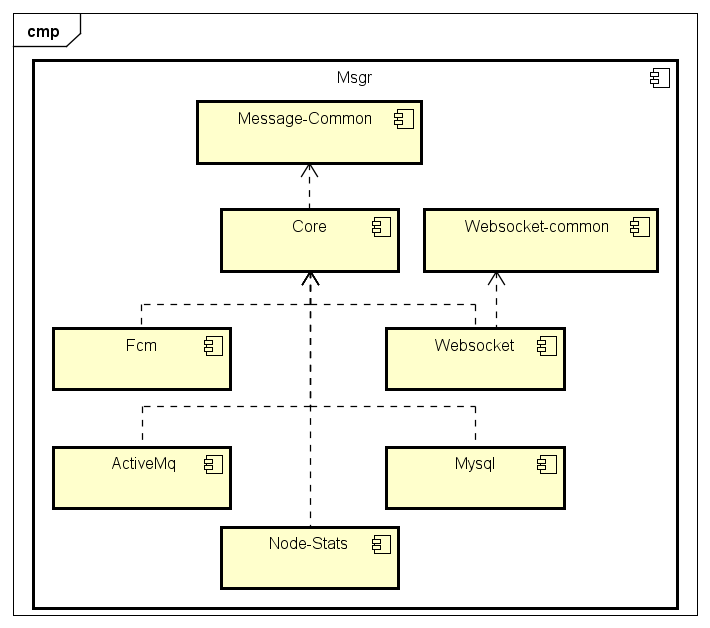
\includegraphics[width=0.7\textwidth]{figures/04_implementation/msgr-project}
    \caption{Modules in the Msgr project and their dependencies on each other}
    \label{fig:msgr-project}
\end{figure}

\subsection{Msgr}
The Msgr project represents the Node application, containing both the system core and modules containing the sample implementation of the modular components of the system. 

The Msgr root project is just a simple Gradle project containing only a Spring Boot application, but no other code. The root project puts together all the individual modules of the application by declaring dependency on its subprojects, the module projects. The project tree, including dependencies between modules can be seen in Figure \ref{fig:msgr-project}. The following subsections further break down and describe the modules.

\subsubsection{Core Module}
The Core Module contains all the interfaces for other modules to implement, which are explained in detail in Sections \ref{design:database-modularity}, \ref{design:platform-modularity}, and \ref{design:mq-modularity}, the application's core business logic, described in Section \ref{design:business-tier}, and several controllers providing core APIs. This section contains a brief description of a selection of the classes contained in the Core Module.

\subsubsection*{Controllers}
The controller package contains three classes: 
\begin{itemize}
    \item \textbf{ConnectionController}, which  serves as the entry point into the system by exposing the \textit{/connect} endpoint. The controller registers the connecting device, based on the \textit{ConnectionRequest} object in the request's payload, and responds with the device's full registration information and a list of addresses of least loaded Nodes.
    
    Example response payload:
    \begin{lstlisting}
    {
      "addresses": [
        "node1.example.com",
        "node2.example.com",
        "node3.example.com"
      ],
      "deviceData": {
        "userId":"user1",
        "userName":"user name",
        "deviceId":"device1",
        "deviceToken":"device 1"
      }
    }
    \end{lstlisting}
    
    \item \textbf{MessageController}, which provides an API for sending messages and notifications through HTTP REST calls by exposing the \textit{/notification} and \textit{/message} endpoints.
    
    \clearpage
    
    \item \textbf{HealthController}, which exposes the \textit{/health} endpoint that is used by the Node Coordinator to check the Node's health and receive Node status data.
    
    Example response payload:
    \begin{lstlisting}
    {
        "load":0.4,
        "memory":58.7
    }
    \end{lstlisting}
\end{itemize}

\subsubsection*{Queue Processors}
The queue package contains classes that perform the processing of messages dequeued from general queues, such as the group and user queues.

\subsubsection*{CoordinatorConnector}
The \textit{CoordinatorConnector} class represents a bean that, at the start of the Spring Application Context, announces the Node to the Node Coordinator, and then caches and refreshes the list of least loaded Nodes from the Coordinator.

\subsubsection*{Services}
The services package contains the \textit{AdapterService} and \textit{MessagingService} classes, which provide most of the core business logic and are described in detail in Section \ref{design:business-tier} \nameref{design:business-tier}.

\subsubsection{Message-Common}
The \textit{Message-Common} module is a simple collection of Data Transfer Objects (DTOs), which serve to encapsulate data sent over APIs, and a few utility methods for working with them. The \textit{Message-Common} module is meant to be used as a library in other projects which use these same classes, such as the \textit{Java-Client}.

\subsubsection{Fcm}
The \textit{Fcm} module contains the adapter implementation for the FCM platform.

\subsubsection{Mysql}
The \textit{Mysql} module contains implementations for the Data Tier modularity interfaces, as described in Section \ref{design:data-layer} \nameref{design:data-layer}.

\subsubsection{Websocket}
The \textit{Websocket} module contains the adapter implementations for the Websocket platform.

\subsubsection{Websocket-Common}
The \textit{Websocket-Common} module contains classes that are shared between the \textit{Websocket} module and the \textit{Java-Client} project.

\subsubsection{ActiveMq}
The \textit{ActiveMq} module contains the implementations of the message queue interfaces for the ActiveMQ platform, along with all message queue related logic.

\subsubsection{Node-Stats}
The \textit{Node-Stats} module exposes the \textit{/stats} endpoint, which provides detailed information on the current state of the Node, including the number of connections to the message queue, bound devices, and more.

Example response payload:
\begin{lstlisting}
{
  "system": {
    "load": 0.272,
    "memory": 37.92
  },
  "totalBoundClients": 0,
  "platformClients": {
    "websocket": 0
  },
  "mq": {
    "totalConnections": 1,
    "sessions": 3,
    "origins": [
      "queue://FCM",
      "queue://q.group.*",
      "queue://q.user.*"
    ]
  }
}
\end{lstlisting}

\subsection{Coordinator}
The Coordinator project represents the Node Coordinator application, which maintains a list of all connected Nodes and performs regular health checks on them. The Coordinator also exposes \textit{/free-nodes} endpoint, which provides the list of \textit{n} least loaded nodes, and a monitor page containing the current status and health of the Coordinator and all its connected Nodes (see Figure \ref{fig:monitor-page}).

\begin{figure}[!ht]
	\centering
	\fbox{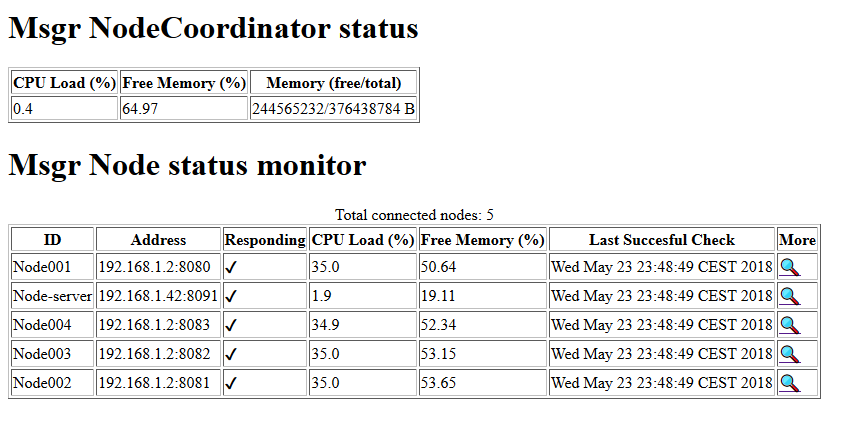
\includegraphics[width=0.9\textwidth]{figures/04_implementation/monitor-page}}
    \caption{Node Coordinator monitor page}
    \label{fig:monitor-page}
\end{figure}

The Coordinator further includes the \textit{Common} module subproject, which contains utility classes for obtaining statistics about the system, such as CPU load and free memory. This module is used as a library in the \textit{Core} module of the Msgr project.

\subsection{Java-Client}
The Java-Client project contains the classes forming the Java platform client library, which is described in detail in Section \ref{design:client-java} \nameref{design:client-java}.

\subsection{Web}
The Web project contains the sample implementation for the Web platform, which consists of a Javascript client library and a web application, called Chattr, which functions as an IM chat that can be used to send and receive messages (see Figure \ref{fig:chattr-web}).

\begin{figure}[!ht]
	\centering
	\fbox{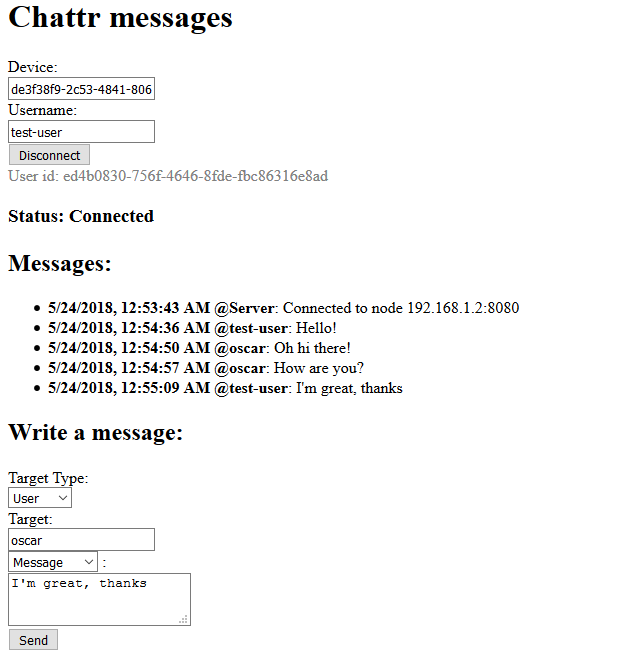
\includegraphics[width=0.9\textwidth]{figures/04_implementation/chattr-web}}
    \caption{Chattr web application screenshot}
    \label{fig:chattr-web}
\end{figure}

\subsection{MsgrChattr}
The MsgrChattr project contains the Android application that is part of the sample implementation for the mobile platform. The app consists of a single screen, or Activity, as they are called in Android terminology, which is able to receive and send messages, showing them in an IM chat fashion (see Figure \ref{fig:chattr-android}). The application uses Google's Firebase Cloud Messaging to receive Android notifications and messages and the Java-Client library to access the system and send messages.

\begin{figure}[!ht]
	\centering
	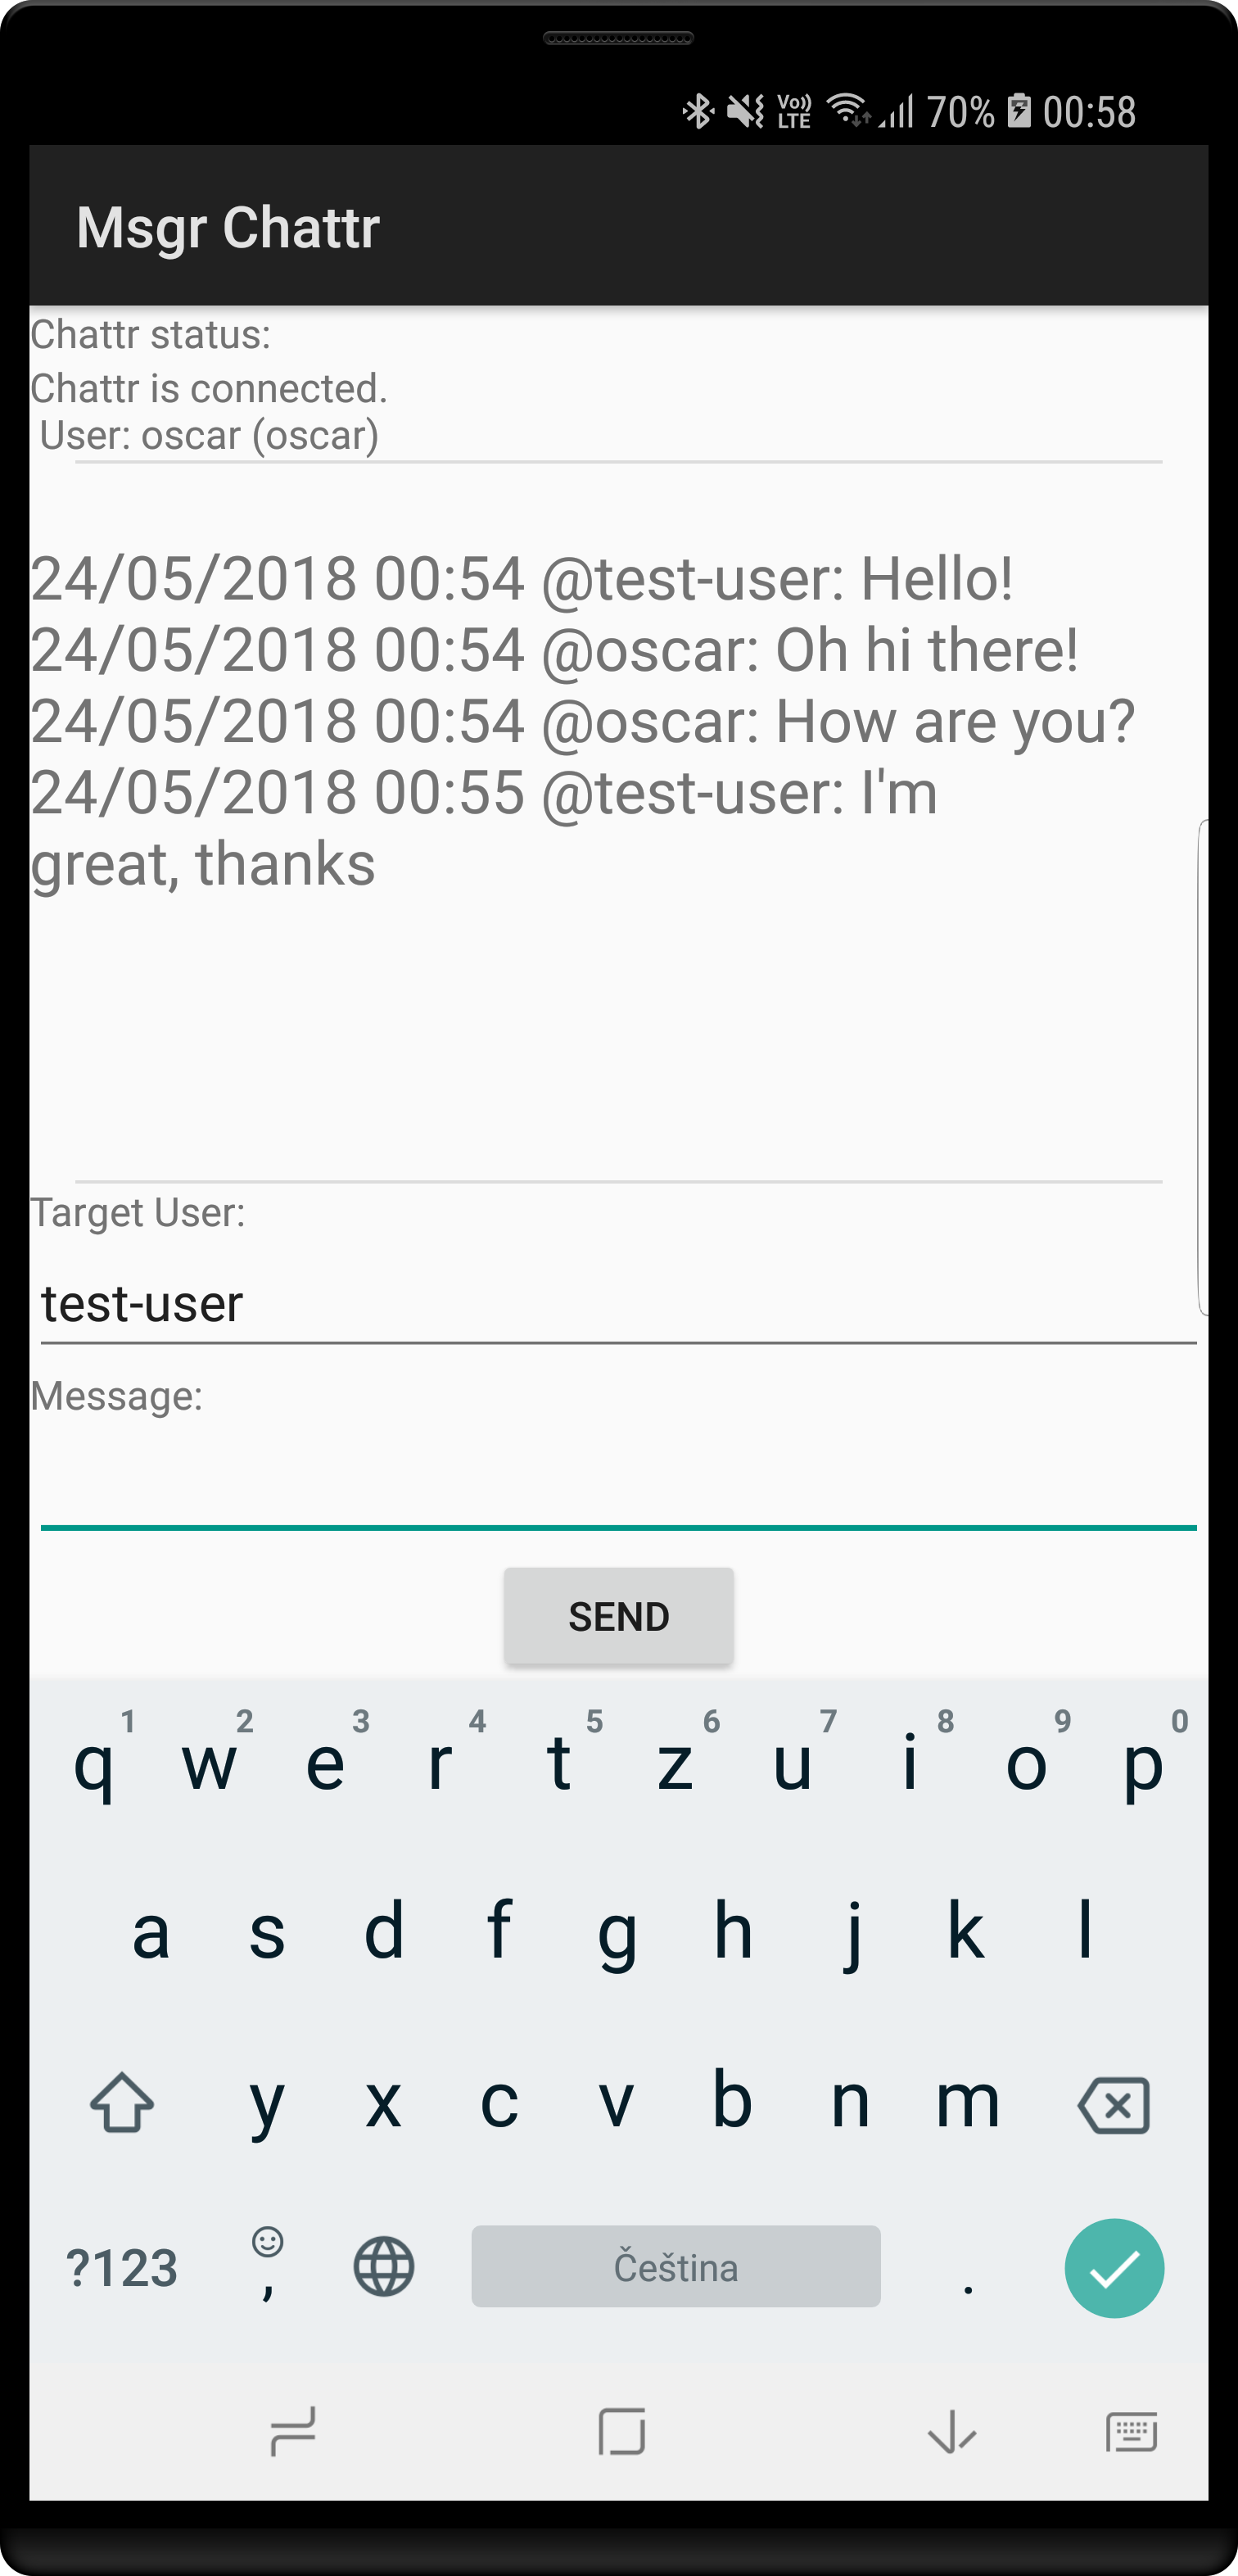
\includegraphics[width=0.5\textwidth]{figures/04_implementation/chattr-android}
    \caption{MsgrChattr Android application screenshot}
    \label{fig:chattr-android}
\end{figure}
